\documentclass[11pt,]{article}
\usepackage[]{mathpazo}
\usepackage{amssymb,amsmath}
\usepackage{ifxetex,ifluatex}
\usepackage{fixltx2e} % provides \textsubscript
\ifnum 0\ifxetex 1\fi\ifluatex 1\fi=0 % if pdftex
  \usepackage[T1]{fontenc}
  \usepackage[utf8]{inputenc}
\else % if luatex or xelatex
  \ifxetex
    \usepackage{mathspec}
  \else
    \usepackage{fontspec}
  \fi
  \defaultfontfeatures{Ligatures=TeX,Scale=MatchLowercase}
\fi
% use upquote if available, for straight quotes in verbatim environments
\IfFileExists{upquote.sty}{\usepackage{upquote}}{}
% use microtype if available
\IfFileExists{microtype.sty}{%
\usepackage{microtype}
\UseMicrotypeSet[protrusion]{basicmath} % disable protrusion for tt fonts
}{}
\usepackage{hyperref}
\PassOptionsToPackage{usenames,dvipsnames}{color} % color is loaded by hyperref
\hypersetup{unicode=true,
            colorlinks=true,
            linkcolor=black,
            citecolor=black,
            urlcolor=black,
            breaklinks=true}
\urlstyle{same}  % don't use monospace font for urls
\usepackage{natbib}
\bibliographystyle{amnat}
\usepackage{graphicx,grffile}
\makeatletter
\def\maxwidth{\ifdim\Gin@nat@width>\linewidth\linewidth\else\Gin@nat@width\fi}
\def\maxheight{\ifdim\Gin@nat@height>\textheight\textheight\else\Gin@nat@height\fi}
\makeatother
% Scale images if necessary, so that they will not overflow the page
% margins by default, and it is still possible to overwrite the defaults
% using explicit options in \includegraphics[width, height, ...]{}
\setkeys{Gin}{width=\maxwidth,height=\maxheight,keepaspectratio}
\IfFileExists{parskip.sty}{%
\usepackage{parskip}
}{% else
\setlength{\parindent}{0pt}
\setlength{\parskip}{6pt plus 2pt minus 1pt}
}
\setlength{\emergencystretch}{3em}  % prevent overfull lines
\providecommand{\tightlist}{%
  \setlength{\itemsep}{0pt}\setlength{\parskip}{0pt}}
\setcounter{secnumdepth}{0}
% Redefines (sub)paragraphs to behave more like sections
\ifx\paragraph\undefined\else
\let\oldparagraph\paragraph
\renewcommand{\paragraph}[1]{\oldparagraph{#1}\mbox{}}
\fi
\ifx\subparagraph\undefined\else
\let\oldsubparagraph\subparagraph
\renewcommand{\subparagraph}[1]{\oldsubparagraph{#1}\mbox{}}
\fi

%%% Use protect on footnotes to avoid problems with footnotes in titles
\let\rmarkdownfootnote\footnote%
\def\footnote{\protect\rmarkdownfootnote}

%%% Change title format to be more compact
\usepackage{titling}

% Create subtitle command for use in maketitle
\providecommand{\subtitle}[1]{
  \posttitle{
    \begin{center}\large#1\end{center}
    }
}

\setlength{\droptitle}{-2em}

  \title{}
    \pretitle{\vspace{\droptitle}}
  \posttitle{}
    \author{}
    \preauthor{}\postauthor{}
    \date{}
    \predate{}\postdate{}
  
\usepackage{fullpage}
\linespread{1.5}
\usepackage{lineno}
\usepackage{caption}
\captionsetup[figure]{font=small,labelformat=empty}

\begin{document}

\vspace*{0.1cm}

\begin{center} \LARGE Appendix S4: \\ Ecological character displacement destabilizes food webs \end{center}

\bigskip

\begin{center} \large Matthew A. Barbour$^{1,2,\ast}$ \normalsize \end{center}

\bigskip

\noindent 1. University of Zurich, Department of Evolutionary Biology
and Environmental Studies, 8057 Zurich, Switzerland;

\noindent 2. University of British Columbia, Department of Zoology,
Vancouver, BC V6T 1Z4, Canada;

\(^\ast\) Corresponding author; e-mail:
\href{mailto:matthew.barbour@ieu.uzh.ch}{\nolinkurl{matthew.barbour@ieu.uzh.ch}}

\bigskip

\emph{Elements}: Figures S1, S2, and S3.

\newpage

\begin{figure}
\centering
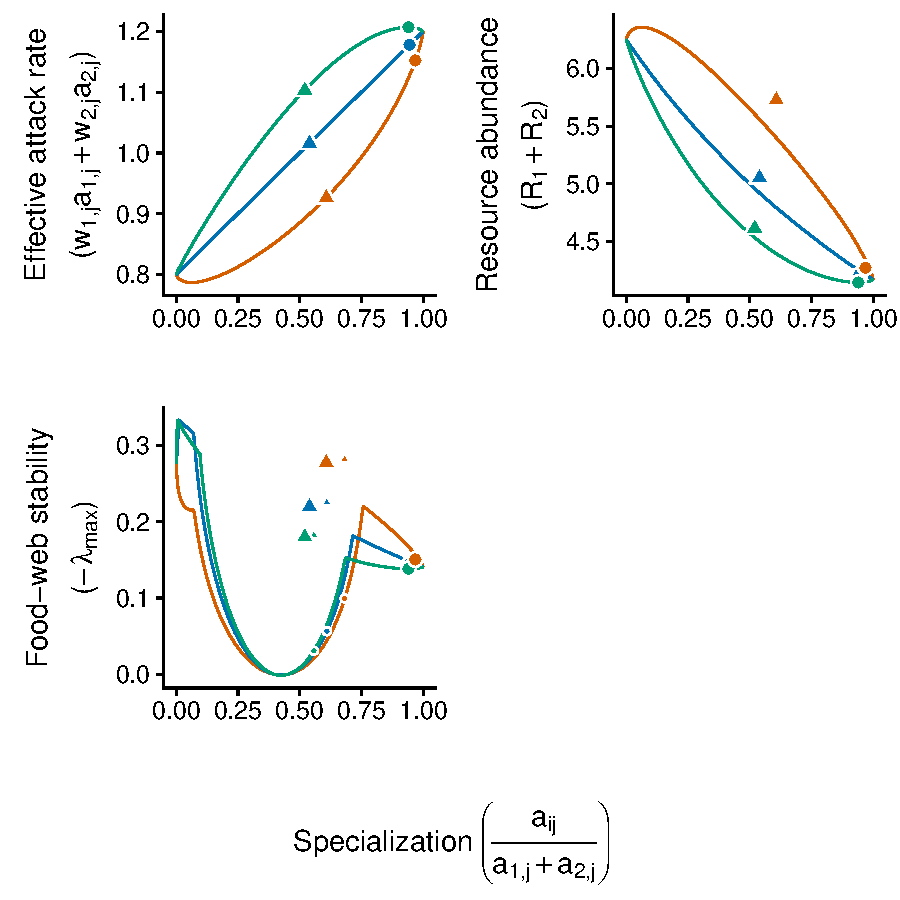
\includegraphics{Figure_ECD_McCann.pdf}
\caption{Figure S1: \textbf{Effect of character displacement when
consumers exhibit a more realistic functional response.} Different line
colors correspond to different tradeoff values (green, \emph{n} = 1.15;
blue, \emph{n} = 1; orange, \emph{n} = 0.85). Large circles (two
consumers) and triangles (one consumer) correspond to the end points of
the eco-evolutionary simulation for \emph{C}\textsubscript{1}, whereas
as small shapes correspond to the starting points (only in stability
panel). This figure illustrates how, regardless of the tradeoff,
character displacement increases the effective attack rate of consumers.
This always resulted in a suppression of resource abundances and
concomitant decrease in food-web stability. Initial parameter and state
variables are given in the main text.}
\end{figure}

\newpage 

\begin{figure}
\centering
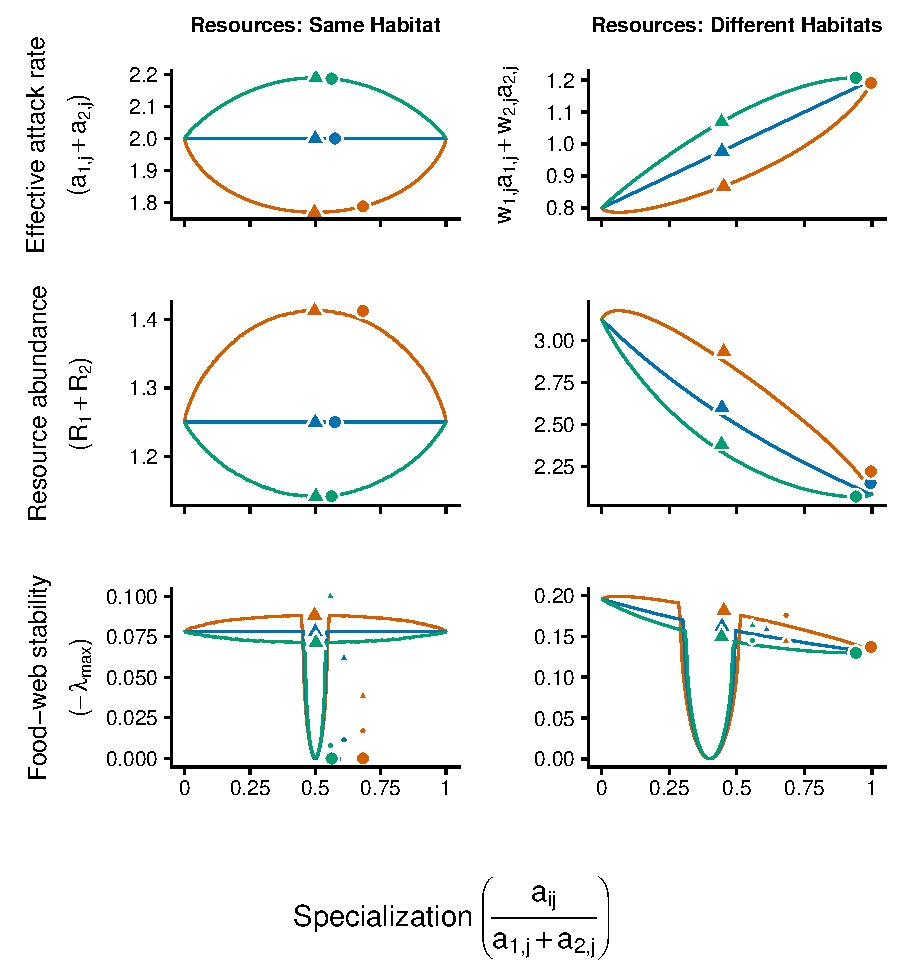
\includegraphics{asymm_figs.pdf}
\caption{Figure S2: \textbf{Robustness to consumer asymmetry}. Lines
show predicted values when both consumers and resources are present.
Different line colors correspond to different tradeoffs in attack rates
(green, \emph{n} = 1.15; blue, \emph{n} = 1; orange, \emph{n} = 0.85).
Large circles (two consumers) and triangles (one consumer) correspond to
the end points of the eco-evolutionary simulation for
\emph{C}\textsubscript{1}, whereas as small shapes correspond to the
starting points (only in stability panels). In both foraging scenarios,
feeding rates increase linearly with resource abundance, but the
equation for effective attack rate is different. The similarity with
fig. 3 (main text) shows that adding an asymmetry in consumer attack
rates does not alter the conclusions reported in the main text. If
anything, it is more likely that an asymmetry will push the system
toward the boundary of stability (note position of large circles in
lower left stability panel). Details of the consumer asymmetry
simulation are given in the main text.}
\end{figure}

\begin{figure}
\centering
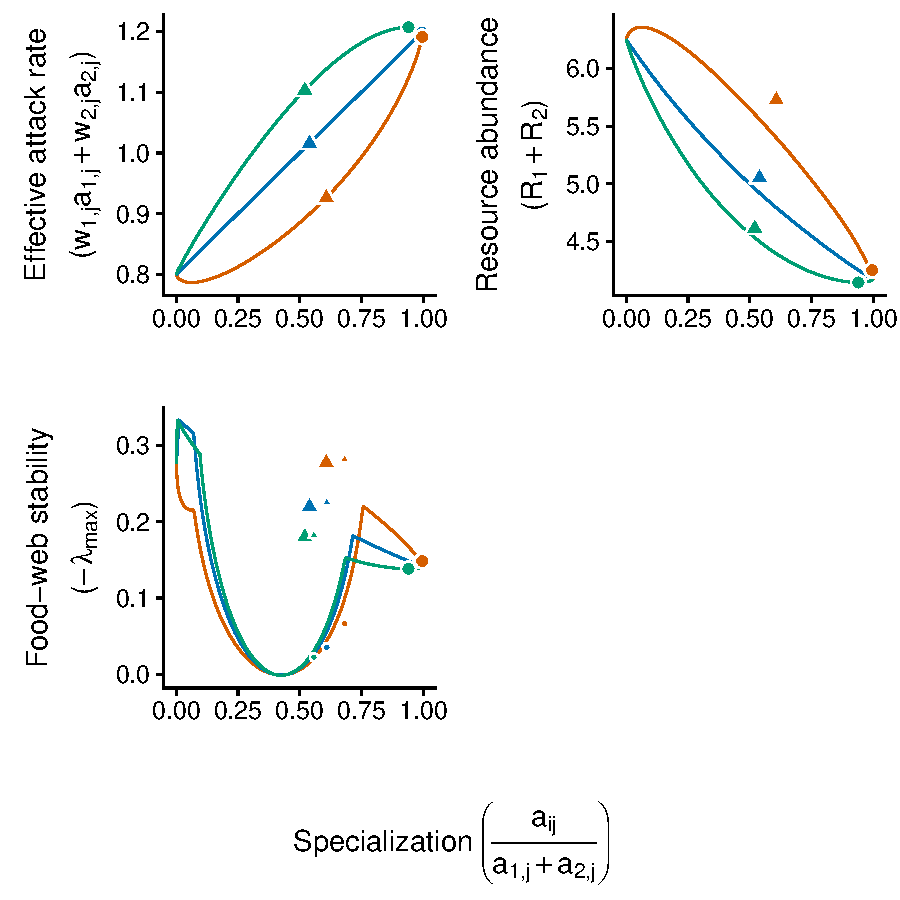
\includegraphics{Figure_ECD_McCann_asymm.pdf}
\caption{Figure S3: \textbf{Robustness to consumer asymmetry when
consumers exhibit a more realistic functional response.} Different line
colors correspond to different tradeoff values (green, \emph{n} = 1.15;
blue, \emph{n} = 1; orange, \emph{n} = 0.85). Large circles (two
consumers) and triangles (one consumer) correspond to the end points of
the eco-evolutionary simulation for \emph{C}\textsubscript{1}, whereas
as small shapes correspond to the starting points. Panel (A) shows how,
regardless of the tradeoff, character displacement increases the
effective attack rate of consumers. This always resulted in a
suppression of resource abundances (B) and concomitant decrease in
food-web stability (C). The similarity with fig. S1 shows that adding an
asymmetry in consumer attack rates does not alter the conclusions
reported in the main text. Details of the consumer asymmetry simulation
are given in the main text.}
\end{figure}

\bibliography{references}


\end{document}
